This proposed new installment of the NEMO detectors series consists of up to 20 tracker-calo modules, each one containing a thin foil of about 5 kg of \bb-decaying material, probably \SE, although other isotopes such as \ND\ or \CA\ are also under consideration. 

A sketch of a SuperNEMO module can be seen in fig.~\ref{fig:snemo}. The source foil, 3 meters high and 4.5 meters long, with a surface density of about 40 mg/cm$^{2}$, is placed in the center of a tracking chamber with overall dimensions of 4 m height, 5 m length and 1 m width. Nine planes of drift cells operating in Geiger mode and a magnetic field of 25 Gauss allow to reconstruct the trajectory and charge of particles crossing the chamber. A calorimeter consisting of blocks of plastic scintillator coupled to low-activity PMTs surrounds the tracking chamber on four sides. Its granularity allows the energy of individual particles to be measured.

%%%%%
\begin{figure}[t!b!]
\begin{center}
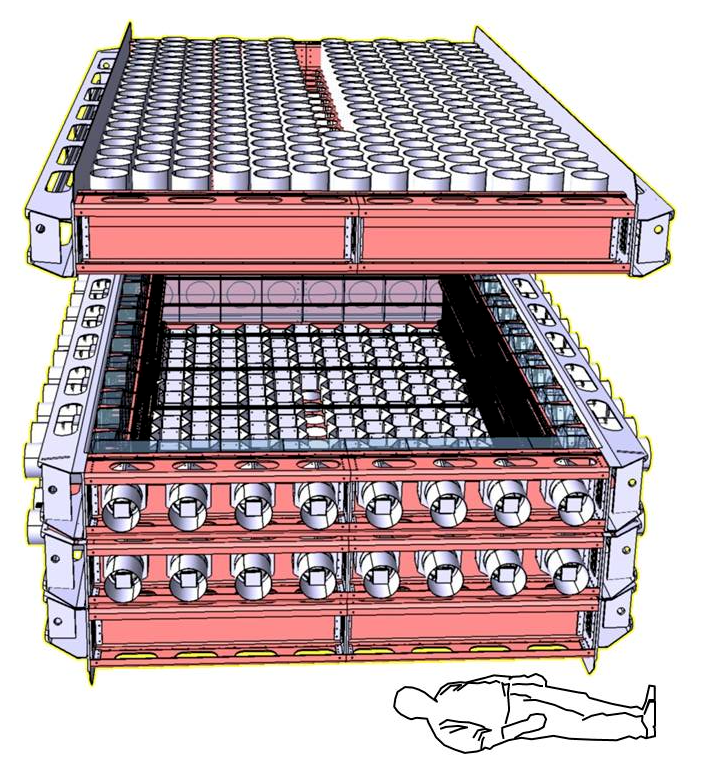
\includegraphics[angle=270,width=0.45\textwidth]{img/snemo-1.eps} \hspace{0.04\textwidth}
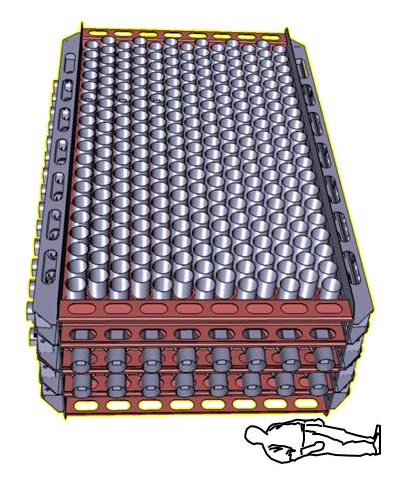
\includegraphics[angle=270,width=0.45\textwidth]{img/snemo-2.eps}
\end{center}
\caption{A SuperNEMO module. The source foil (not shown) is placed in the center of a tracking volume consisting of drift cells operating in Geiger mode. The tracking volume is surrounded by calorimetry consisting of scintillator blocks connected to PMTs (grey). The support frame is shown in red.} \label{fig:snemo}
\end{figure}
%%%%%

The physics case of SuperNEMO relies on several significant improvements over the NEMO-3 detector performance \cite{Shitov:2010nt}. The energy resolution is expected to be 7\% FWHM at 1 MeV, a factor of 2 better than in NEMO-3. Such a resolution has been attained with a 28 cm hexagonal PVT scintillator directly coupled to a 8-inch PMT \cite{Freshville:2011zz}. The detection efficiency of SuperNEMO is estimated by means of simulation to be about 30\%, almost a factor of 2 better than in NEMO-3. As far as the backgrounds are concerned, SuperNEMO goals require an impressive improvement in the purification (both chemical and via distillation methods) of the source foils. In particular, \BI\ and \TL\ contamination in \SE\ foils are to be reduced by factors of 50 and 170, respectively. A dedicated setup, the BiPo detector, installed in the Laboratorio Subterr\'aneo de Canfranc (LSC), will measure the radiopurity of the foils in order to make sure that the required levels are achieved. Finally, in order to decrease radon gas levels in the tracking chamber down to negligible levels ($<$0.15 mBq/m$^3$ ), a reduction of at least a factor of 40 with respect to NEMO-3 is needed. 

The first SuperNEMO module, called the demonstrator, will be the first step from R\&D to construction with the aims to demonstrate the feasibility of large scale mass production, to measure the backgrounds (especially from radon emanation), and to finalize the detector design. The demonstrator will be installed in the space previously occupied by the NEMO-3 detector at the Modane Underground Laboratory.

The current plans of the SuperNEMO Collaboration for the following: (a) demonstrator construction, 2010--2012; (b) demonstrator physics run start-up, 2013; and (c) full detector construction start-up, 2014. 